\begin{titlepage}
  % HACK for two-sided documents: ignore binding correction for cover page.
  % Adapted from Markus Kohm's KOMA-Script titlepage=firstiscover handling.
  % See http://mirrors.ctan.org/macros/latex/contrib/koma-script/scrkernel-title.dtx,
  % \maketitle macro.
  \oddsidemargin=\evensidemargin\relax
  \textwidth=\dimexpr\paperwidth-2\evensidemargin-2in\relax
  \hsize=\textwidth\relax

  \centering

  \IfFileExists{logos/tum_logo_transparent.png}{%
    
\includegraphics[height=20mm]{logos/tum_logo_transparent.png}
  }{%
    \vspace*{20mm}
  }

  \vspace{10mm}
  \begin{spacing}{1.5}
    {\huge\MakeUppercase{\getFaculty{}}}
  \end{spacing}

  \vspace{5mm}
  {\large\MakeUppercase{\getUniversity{}}}\\

  \vspace{15mm}
  {\Large \getDoctype{}}

  \vspace{25mm}
  {\huge\bfseries \getTitle{}}

  \vspace{15mm}
  {\LARGE \getAuthor{}}

  \IfFileExists{logos/tum_informatik_logo.png}{%
    \vfill{}
    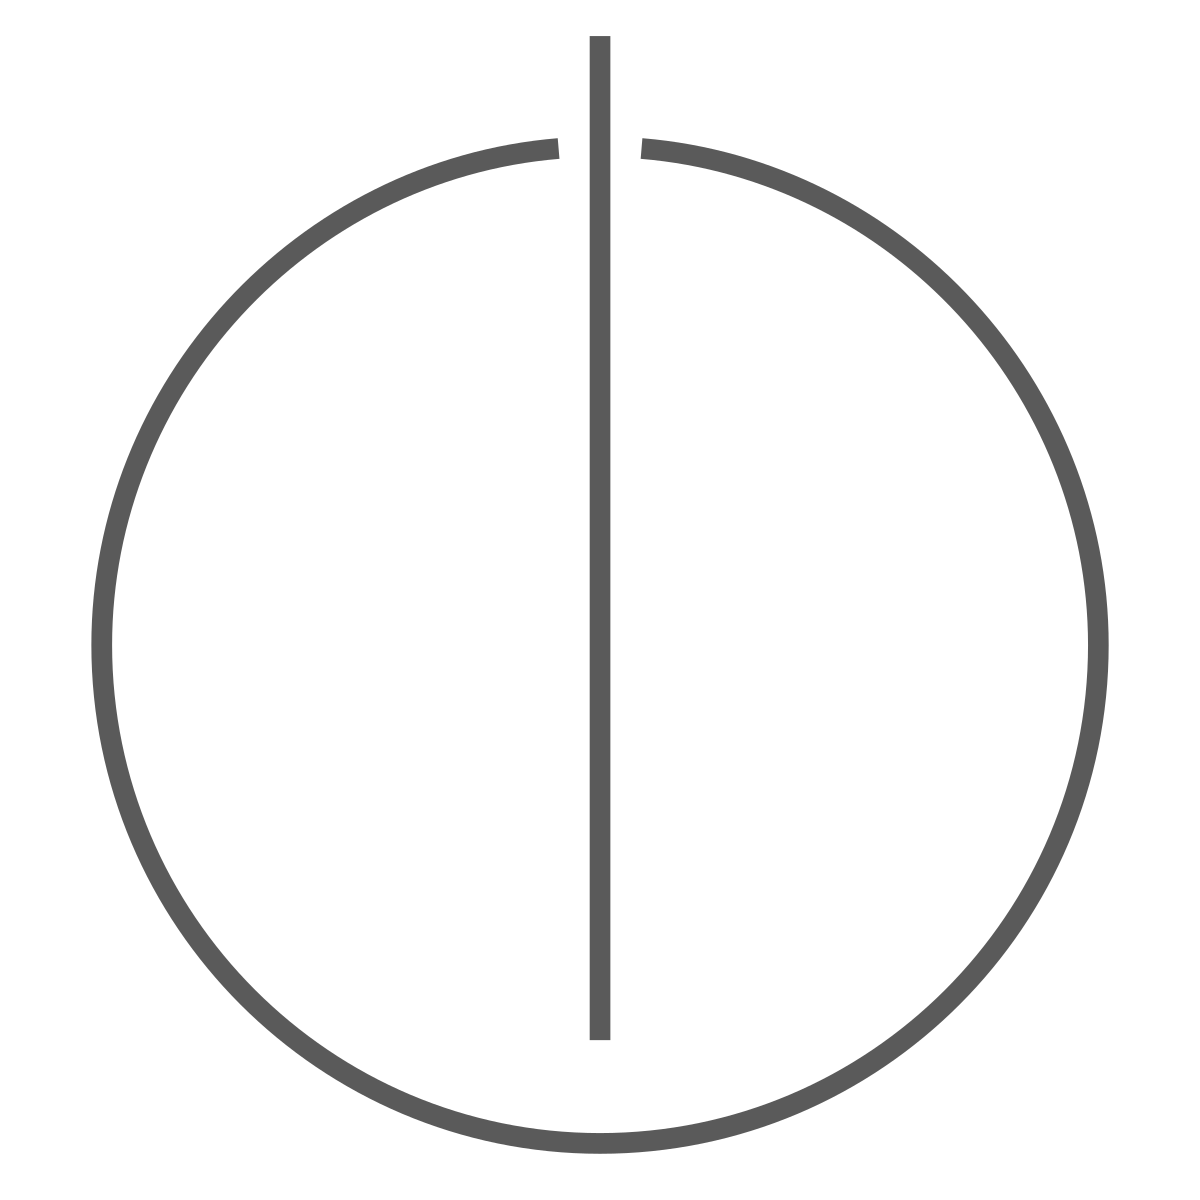
\includegraphics[height=20mm]{logos/tum_informatik_logo.png}
  }{}
\end{titlepage}
